\subsection{Estimating the decay rate of the Legendre coefficients}

Having tested the \textit{h-adaptive} refinement capabilities for this $DG$ implementation, the next and final step is to implement \textit{p-adaptive} refinement using a test of analyticity.

\cite{Eibner2007} Since the solution is represented by the coefficients of Legendre polynomials, analyticity can be assessed by evaluating their rate of decay.

Given \eqref{decomposition}, the following relation can be written for every element $K$:

\begin{gather}
    u^{k, ij}_{h, K} = c_{ij} \phi_{ij} \quad \Forall i, j : i + j = k.
\end{gather}

Assuming smoothness for $u^k_{h, K}$, the following holds:

\begin{gather}
    \Exists a_K, b_K \in \R : c_{ij} \approx a_K e^{-b_K (i + j)}.
\end{gather}

An estimate of $b_K$ through a linear fit of $\log(\lvert c_{ij} \rvert)$ is the key to choosing \textit{p-refinement} over \textit{h-refinement}. In fact, $u^k_{h, K}$ is said to be smooth if $b_K$ exceeds a certain threshold, fixed to $1.0$ in the following numerical tests.

The marking strategy is slightly modified so that the elements $K$ to be refined are chosen in the following way:

\begin{gather}
    \eta_K^2 > \sigma \bar{\eta}^2,
\end{gather}

where:

\begin{gather}
    \bar{\eta}^2 = \frac{1}{\lvert \Tau \rvert} \sum_{K \in \Tau} \eta_K^2.
\end{gather}

\cite{Eibner2007} The expected convergence rates over the L-shaped domain for a singularity-bearing solution and the square domain for a smooth, albeit pathological, solution are:

\begin{gather} 
    \lVert u - u^k_h \rVert_{DG, \, \text{Square}} \approx a \, e^{-b \, \text{DOFs}^{1/2}}, \label{square-hp} \\
    \lVert u - u^k_h \rVert_{DG, \, \text{L-shape}} \approx a \, e^{-b \, \text{DOFs}^{1/3}}. \label{lshape-hp}
\end{gather}

\newpage
\subsubsection{Errors}

Tests with an initial polynomial degree of $k_0 = 1$ exhibit exponential error trends, confirming both \eqref{square-hp} and \eqref{lshape-hp}.

\begin{figure}[!ht]
    \begin{subfigure}[b]{0.45\textwidth}
		% HP v DOFs template for TikZ.

\begin{tikzpicture}
\begin{axis}[
    xlabel={$DOFs^{1/2}$}, % Edit if needed.
    legend pos=north east,
    ymode=log
]

\addplot[solarized-base02, mark=*] coordinates {(8.660254037844387,2.1812) (10.099504938362077,5.27744) (13.784048752090222,6.89851) (17.578395831246947,4.49653) (24.124676163629637,2.12222) (30.95157508108432,0.855475) (34.45286635390443,0.488443) (39.26830783214372,0.379788) (46.36809247747852,0.222617) (55.758407437802596,0.11514) (64.43601477434805,0.0760571) (75.34586916347837,0.0460142)};
\addlegendentry{$DG$ Error}

\end{axis}
\end{tikzpicture}
	\end{subfigure}
	\hfill
	\begin{subfigure}[b]{0.45\textwidth}
		% HP v DOFs template for TikZ.

\begin{tikzpicture}
\begin{axis}[
    xlabel={$DOFs^{1/2}$}, % Edit if needed.
    legend pos=north east,
    ymode=log
]

\addplot[solarized-base02, mark=*] coordinates {(19.364916731037084,2.12045) (20.566963801203133,6.75433) (22.64950330581225,5.0392) (28.635642126552707,1.86658) (33.704599092705436,0.525591) (38.3275357934736,0.303298) (46.04345773288535,0.196046) (57.3149195236284,0.116661) (65.0,0.0525396) (72.40856302952021,0.0318316)};
\addlegendentry{$DG$ Error}

\end{axis}
\end{tikzpicture}
	\end{subfigure}
    \caption{$DG$ error versus $DOFs^{1/2}$ on a sequence of \textit{hp-adaptively} refined meshes over a square domain. $k_0 = 1$, $N_0 = 25$ (left) and $N_0 = 125$ (right).}
\end{figure}

\begin{figure}[!ht]
    \begin{subfigure}[b]{0.45\textwidth}
		% HP v DOFs template for TikZ.

\begin{tikzpicture}
\begin{axis}[
    xlabel={$DOFs^{1/3}$}, % Edit if needed.
    legend pos=north east,
    ymode=log
]

\addplot[solarized-base02, mark=*] coordinates {(4.217163326508746,0.191755) (4.672328728355259,0.255398) (5.0132979349645845,0.248801) (5.383212612087283,0.291174) (5.708267473384861,0.328607) (6.832771452246442,0.404871) (9.878530490026034,0.485699) (12.69507321245234,0.659013) (14.55901434377428,0.230073) (15.921490395218942,0.122269) (16.623800957486996,0.098664) (17.340316055801914,0.0495985) (17.714635665253457,0.0495794) (18.10839938601742,0.0283923) (18.477938151928672,0.0126687) (19.10925056502305,0.00835058) (20.20211721754757,0.00451385) (20.823924640400417,0.00216312) (21.4106622851008,0.00136207) (22.436197851201577,0.00072339)};
\addlegendentry{$DG$ Error}

\end{axis}
\end{tikzpicture}
	\end{subfigure}
	\hfill
	\begin{subfigure}[b]{0.45\textwidth}
		% HP v DOFs template for TikZ.

\begin{tikzpicture}
\begin{axis}[
    xlabel={$DOFs^{1/3}$}, % Edit if needed.
    legend pos=north east,
    ymode=log
]

\addplot[solarized-base02, mark=*] coordinates {(7.211247851537041,0.110732) (7.594363318174861,0.137827) (7.856828007847996,0.135903) (8.14325284978472,0.138095) (8.349125609133615,0.132241) (9.057248245324264,0.126807) (9.77497432636947,0.104464) (11.347061411356195,0.127274) (12.535896814815494,0.080649) (14.044078760203224,0.0184031) (14.830688695146508,0.0266482) (15.454252904182171,0.0302544) (15.975222064844958,0.0142437) (16.880359523050902,0.0118758) (17.72737313911207,0.00729791) (18.257612386946448,0.00512641) (18.86141077038746,0.00483127) (19.51762596542329,0.00280033) (21.299561365474005,0.00152487) (22.75930465103004,0.000784873)};
\addlegendentry{$DG$ Error}

\end{axis}
\end{tikzpicture}
	\end{subfigure}
    \caption{$DG$ error versus $DOFs^{1/3}$ on a sequence of \textit{hp-adaptively} refined meshes over an L-shaped domain. $k_0 = 1$, $N_0 = 25$ (left) and $N_0 = 125$ (right).}
\end{figure}

\newpage

Tests with an initial polynomial degree of $k_0 = 3$ exhibit an exponential error trend earlier than those with $k_0 = 1$, which is significant. However, this trend later deviates, most likely due to the worse ill-conditioning of $\MA$.

\begin{figure}[!ht]
    \begin{subfigure}[b]{0.45\textwidth}
		% HP v DOFs template for TikZ.

\begin{tikzpicture}
\begin{axis}[
    xlabel={$DOFs^{1/2}$},
    legend pos=north east,
    ymode=log
]

\addplot[solarized-base02, mark=*] coordinates {(15.811388300841896,7.96311) (20.85665361461421,6.46708) (25.592967784139454,2.88996) (35.14256678161116,0.972308) (37.76241517699841,0.28022) (39.08964057138413,0.129849) (44.181444068749045,0.083698) (53.786615435440815,0.0436296) (62.120849961989414,0.0214149) (72.29799443968,0.00874589) (85.28188553262645,0.00475347) (100.53854982045445,nan)};
\addlegendentry{$DG$ Error}

\end{axis}
\end{tikzpicture}
	\end{subfigure}
	\hfill
	\begin{subfigure}[b]{0.45\textwidth}
		% HP v DOFs template for TikZ.

\begin{tikzpicture}
\begin{axis}[
    xlabel={$DOFs^{1/2}$}, % Edit if needed.
    legend pos=north east,
    ymode=log
]

\addplot[solarized-base02, mark=*] coordinates {(35.35533905932738,5.22824) (39.370039370059054,2.40924) (44.10215414239989,0.444165) (47.37087712930804,0.152757) (52.25897052181568,0.069876) (60.37383539249432,0.0245913) (70.95773389842716,0.0112348) (79.93122043357026,0.00450677) (85.00588214941364,0.00190181) (94.43516294262429,0.000971294) (101.79390944452423,0.000363691) (112.95574354586844,0.000103198)};
\addlegendentry{$DG$ Error}

\end{axis}
\end{tikzpicture}
	\end{subfigure}
    \caption{$DG$ error versus $DOFs^{1/2}$ on a sequence of \textit{hp-adaptively} refined meshes over a square domain. $k_0 = 3$, $N_0 = 25$ (left) and $N_0 = 125$ (right).}
\end{figure}

\begin{figure}[!ht]
    \begin{subfigure}[b]{0.45\textwidth}
		% HP v DOFs template for TikZ.

\begin{tikzpicture}
\begin{axis}[
    xlabel={$DOFs^{1/3}$},
    legend pos=north east,
    ymode=log
]

\addplot[solarized-base02, mark=*] coordinates {(6.299605249474365,0.220458) (6.46330407009565,0.213463) (7.230426792525689,0.147802) (8.434326653017491,0.0864727) (9.205164082515887,0.063222) (9.86484829732188,0.0473818) (10.446439268223186,0.0367468) (10.969613104865235,0.0304151) (11.447142425533317,0.0274114) (11.974482814936371,0.0241808) (13.103706971044481,0.0156641)};
\addlegendentry{$DG$ Error}

\end{axis}
\end{tikzpicture}
	\end{subfigure}
	\hfill
	\begin{subfigure}[b]{0.45\textwidth}
		% HP v DOFs template for TikZ.

\begin{tikzpicture}
\begin{axis}[
    xlabel={$DOFs^{1/3}$}, % Edit if needed.
    legend pos=north east,
    ymode=log
]

\addplot[solarized-base02, mark=*] coordinates {(10.772173450159418,0.119546) (10.899918636993316,0.114459) (10.999999999999998,0.107735) (11.408857382284173,0.0922831) (11.859471855163267,0.054963) (12.548610714822335,0.0287119) (13.130828854692274,0.0188226) (13.651248393114228,0.0130834) (14.134753229443907,0.00993888) (14.596659021604594,0.00705952) (15.032522029472554,0.00629695) (15.482116036543895,0.00537315) (15.943813338821663,0.0052198) (16.46180328837959,0.00269895) (16.993076765677035,0.00218449) (18.410328165031775,0.00149923) (19.952386738818262,0.000945982) (21.524220046443375,0.000730821)};
\addlegendentry{$DG$ Error}

\end{axis}
\end{tikzpicture}
	\end{subfigure}
    \caption{$DG$ error versus $DOFs^{1/3}$ on a sequence of \textit{hp-adaptively} refined meshes over an L-shaped domain. $k_0 = 3$, $N_0 = 25$ (left) and $N_0 = 125$ (right).}
\end{figure}

\newpage
\subsubsection{Meshes}

\begin{figure}[!ht]
	\centering
    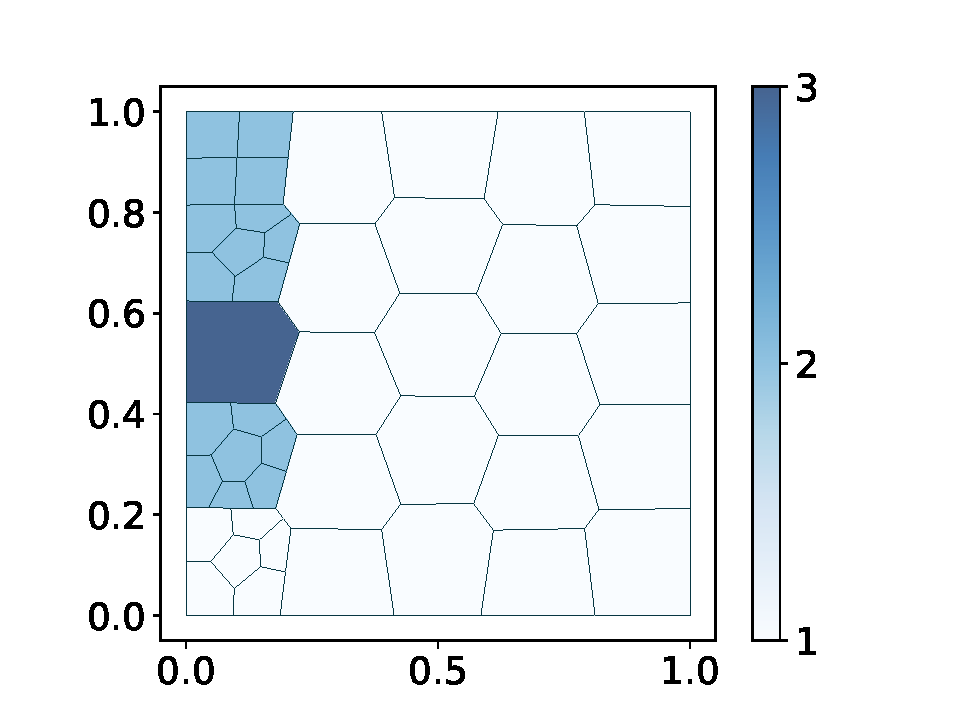
\includegraphics[width=5.5cm]{meshes/adaptive/square_hp_1_2.pdf}
	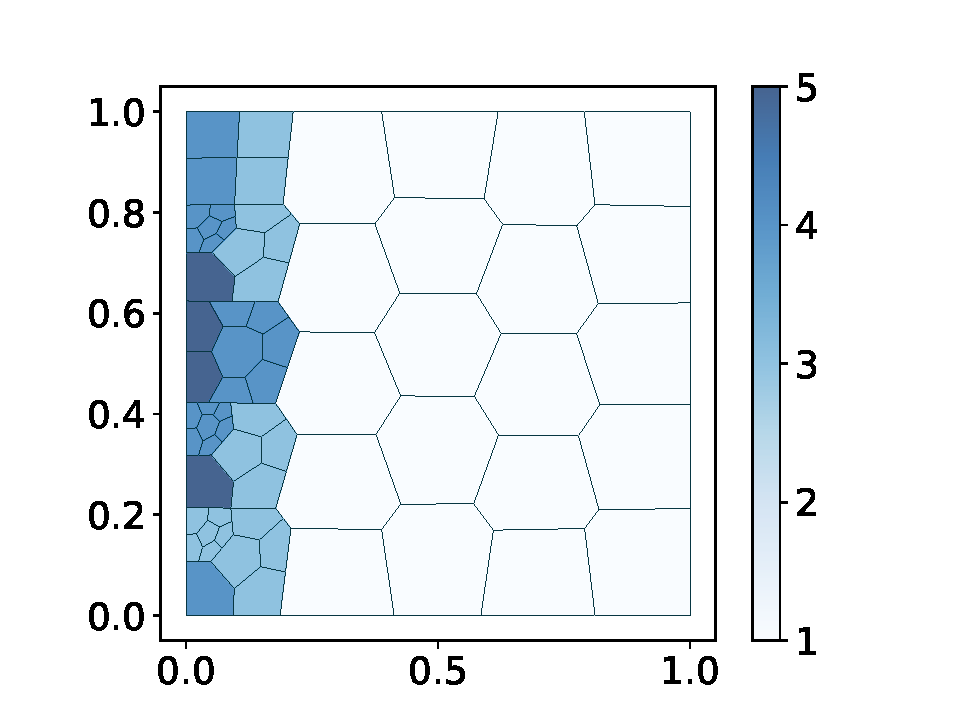
\includegraphics[width=5.5cm]{meshes/adaptive/square_hp_1_5.pdf}
	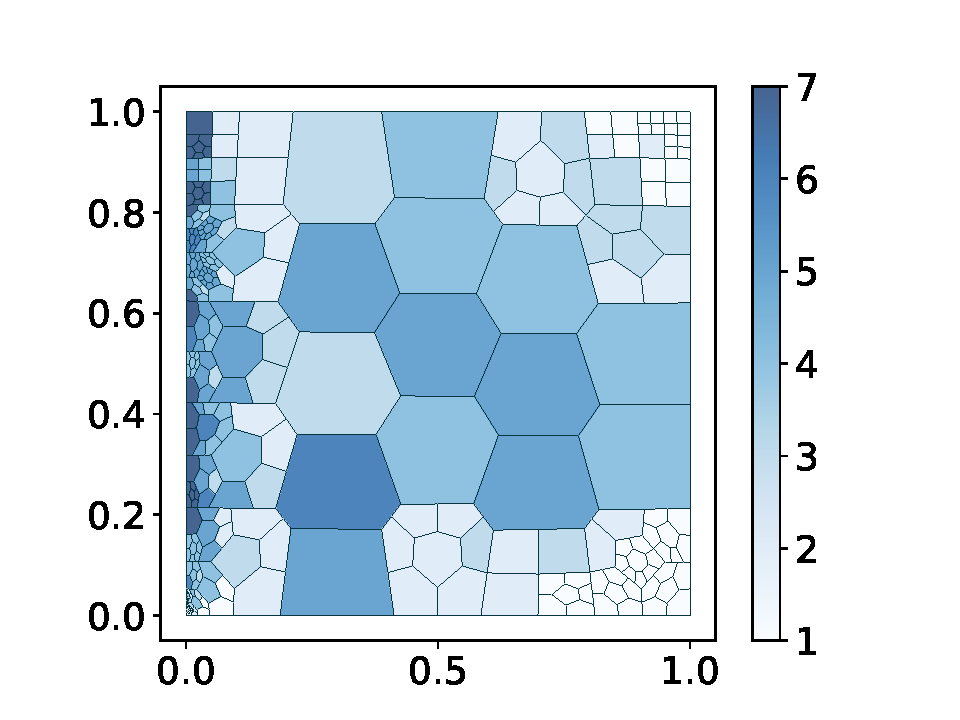
\includegraphics[width=5.5cm]{meshes/adaptive/square_hp_1_10.pdf}
    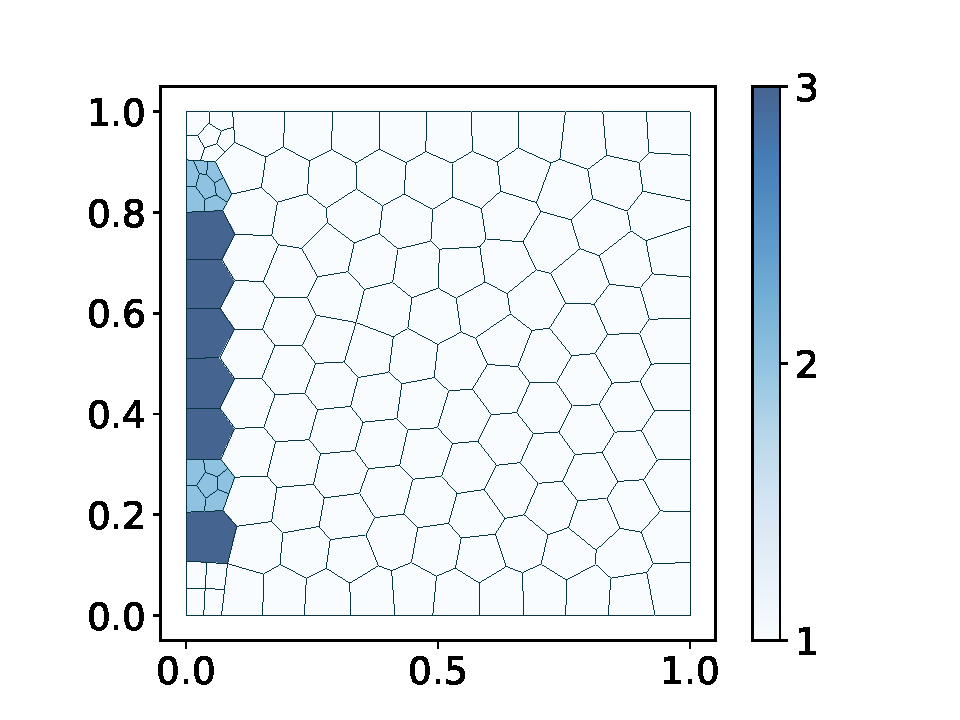
\includegraphics[width=5.5cm]{meshes/adaptive/square_hp_125_1_2.pdf}
	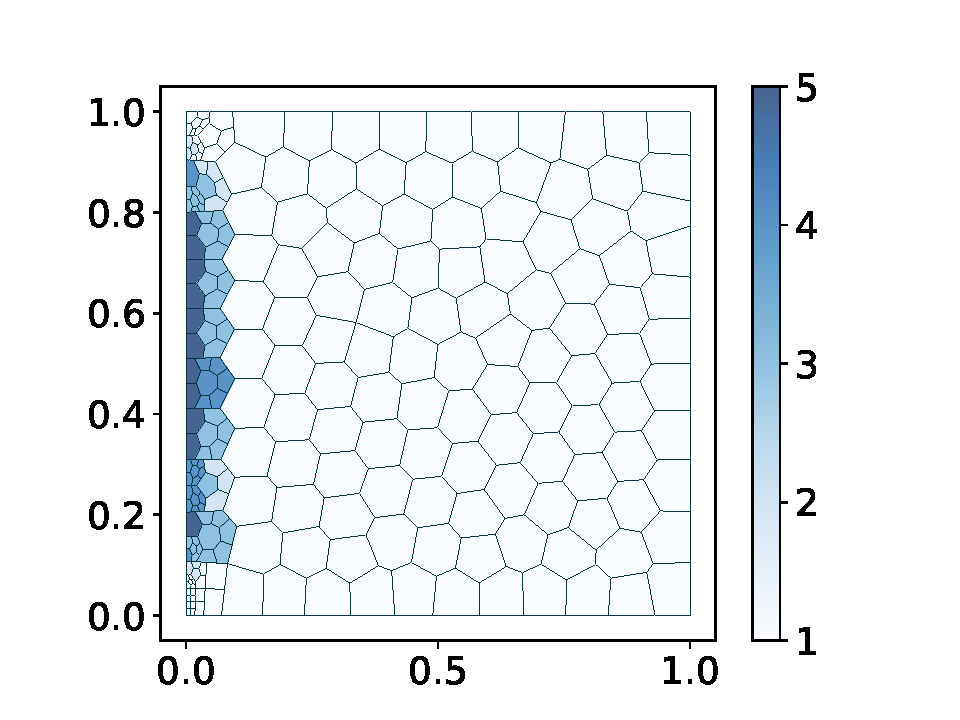
\includegraphics[width=5.5cm]{meshes/adaptive/square_hp_125_1_5.pdf}
	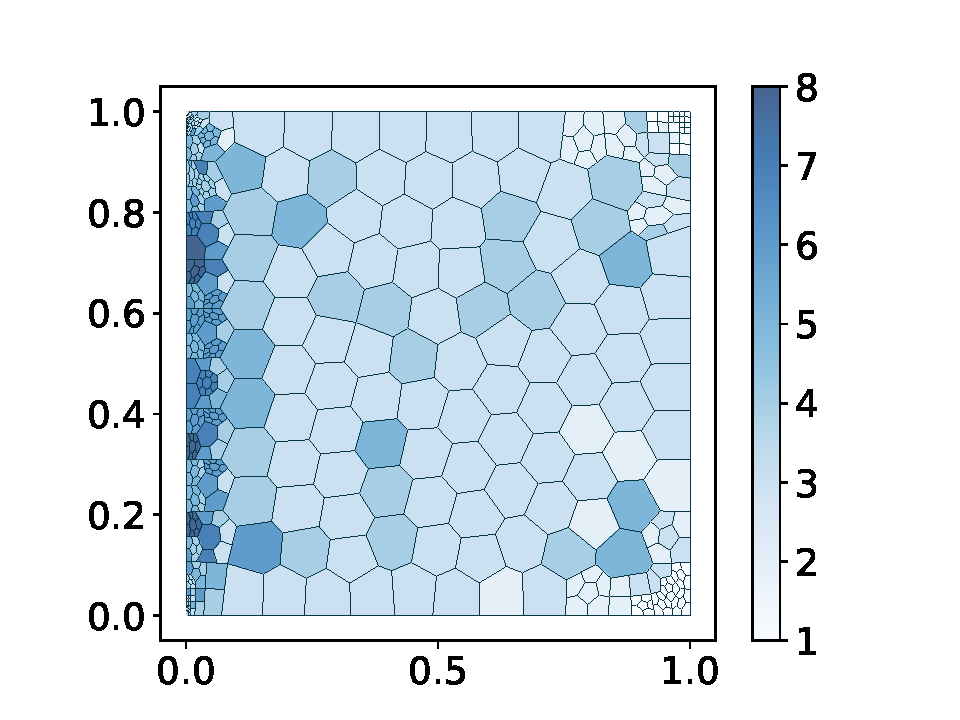
\includegraphics[width=5.5cm]{meshes/adaptive/square_hp_125_1_10.pdf}
    \caption{Square mesh after 2, 5, and 10 refinements. $k_0 = 1$, $N_0 = 25$ (top) and $N_0 = 125$ (bottom).}
\end{figure}

\begin{figure}[!ht]
	\centering
	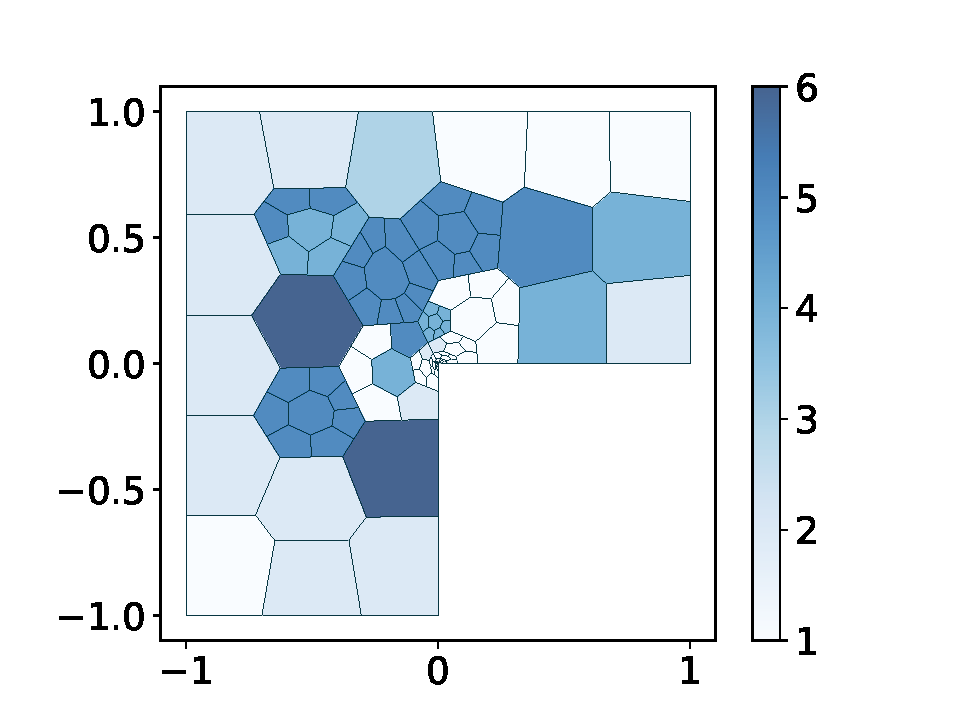
\includegraphics[width=5.5cm]{meshes/adaptive/lshape_hp_1_5.pdf}
	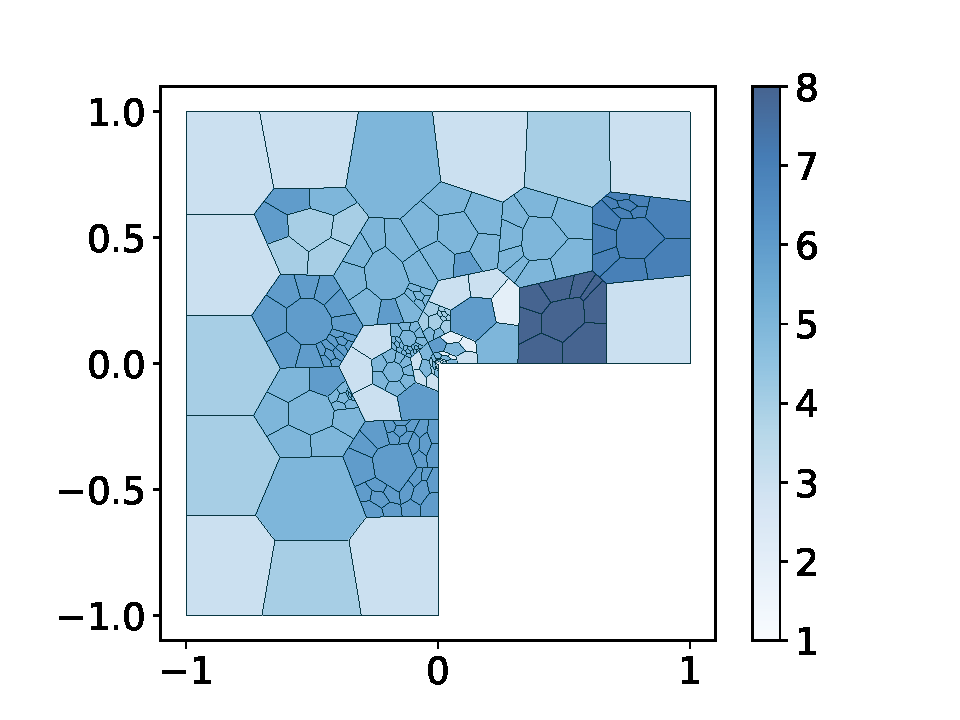
\includegraphics[width=5.5cm]{meshes/adaptive/lshape_hp_1_10.pdf}
	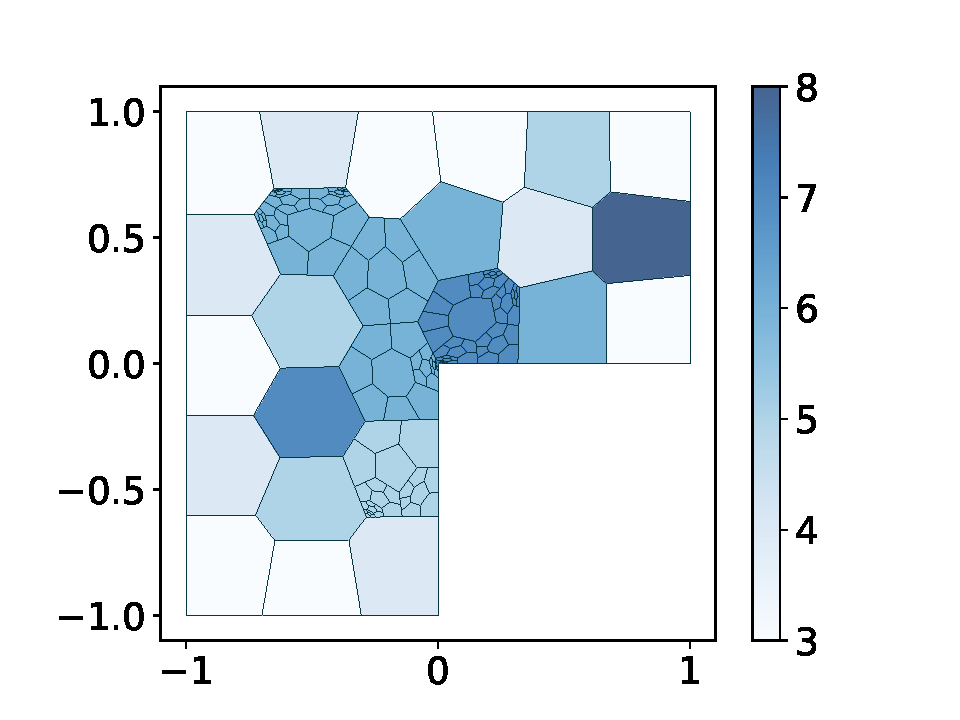
\includegraphics[width=5.5cm]{meshes/adaptive/lshape_hp_1_15.pdf}
    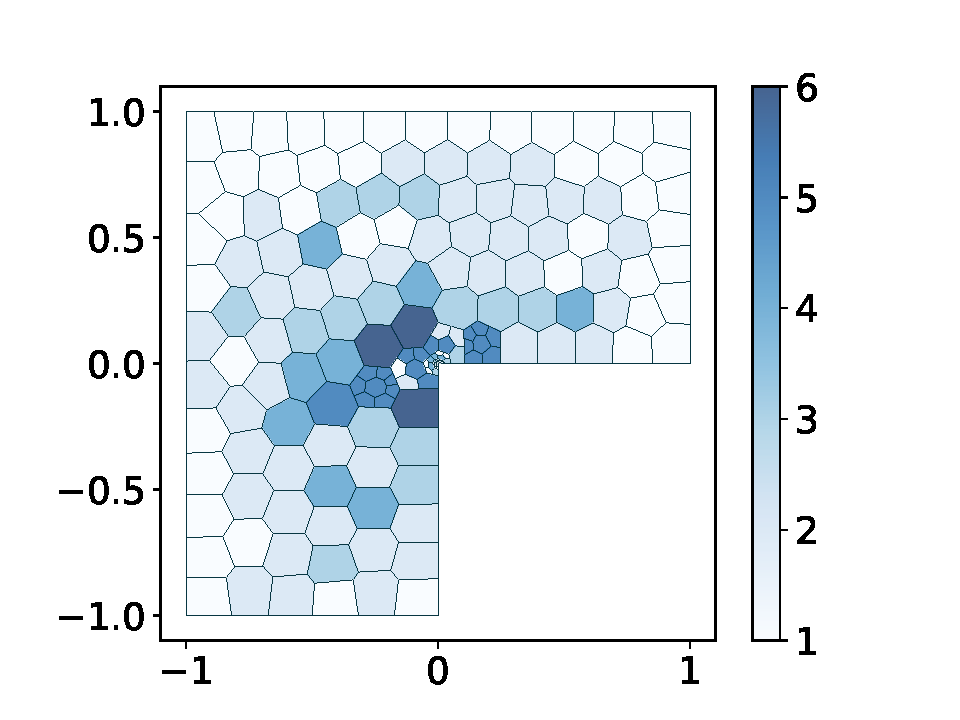
\includegraphics[width=5.5cm]{meshes/adaptive/lshape_hp_125_1_5.pdf}
	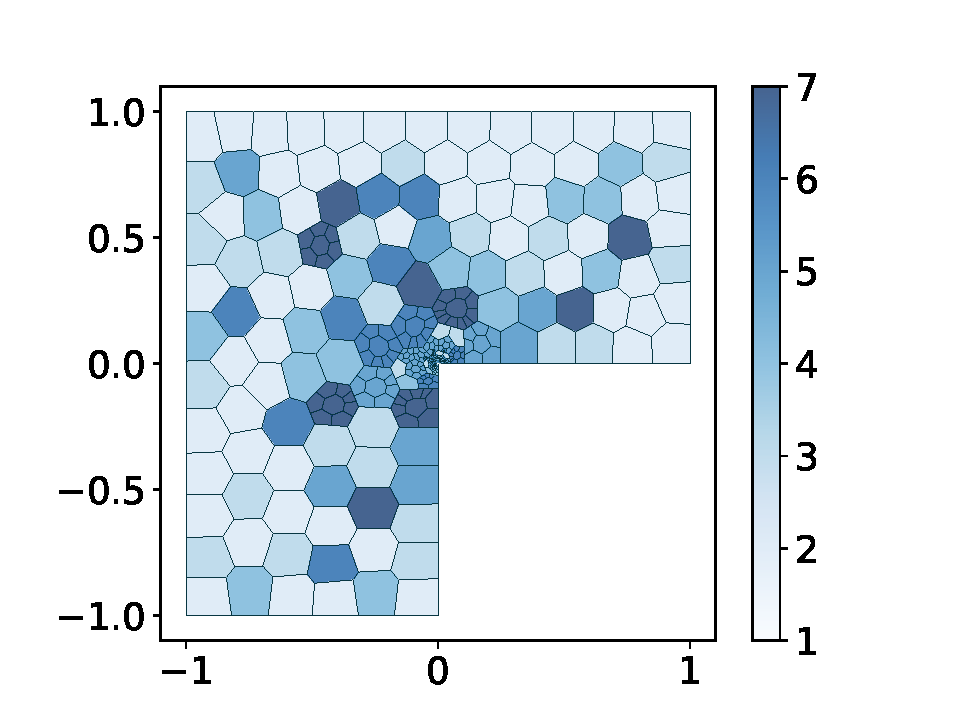
\includegraphics[width=5.5cm]{meshes/adaptive/lshape_hp_125_1_10.pdf}
	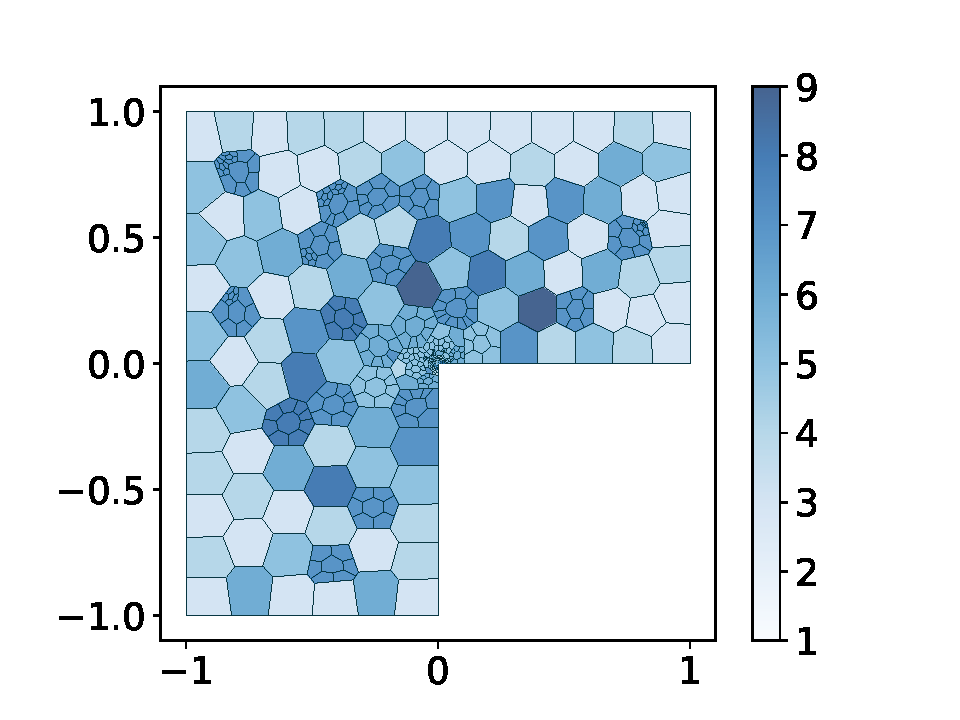
\includegraphics[width=5.5cm]{meshes/adaptive/lshape_hp_125_1_15.pdf}
    \caption{L-shaped mesh after 2, 5, and 10 refinements. $k_0 = 1$, $N_0 = 25$ (top) and $N_0 = 125$ (bottom).}
\end{figure}

\newpage

\begin{figure}[!ht]
	\centering
    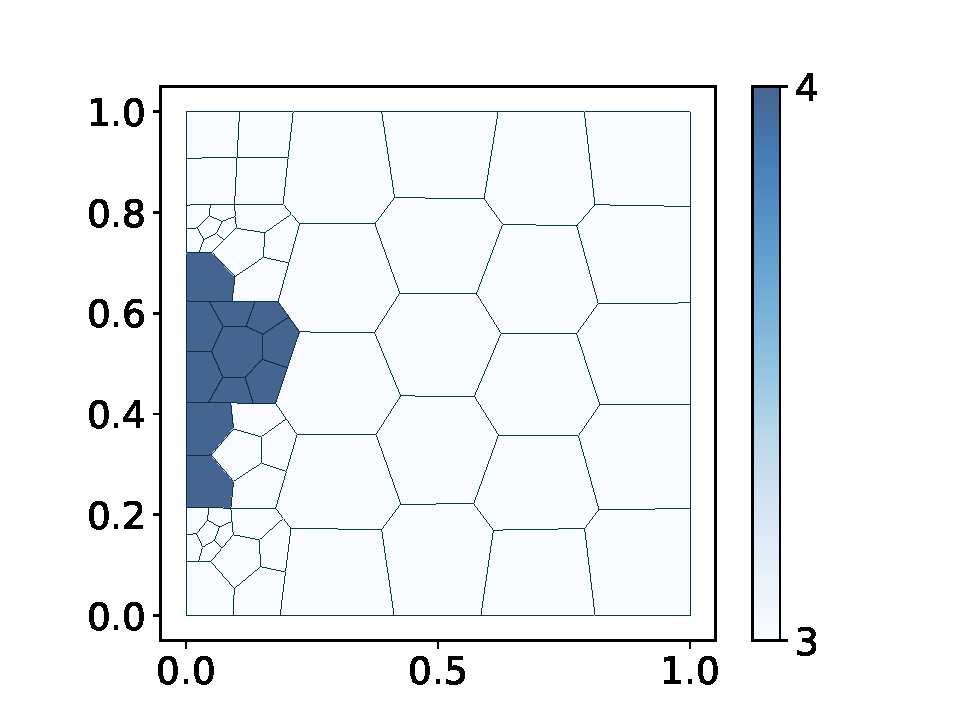
\includegraphics[width=5.5cm]{meshes/adaptive/square_hp_2.pdf}
	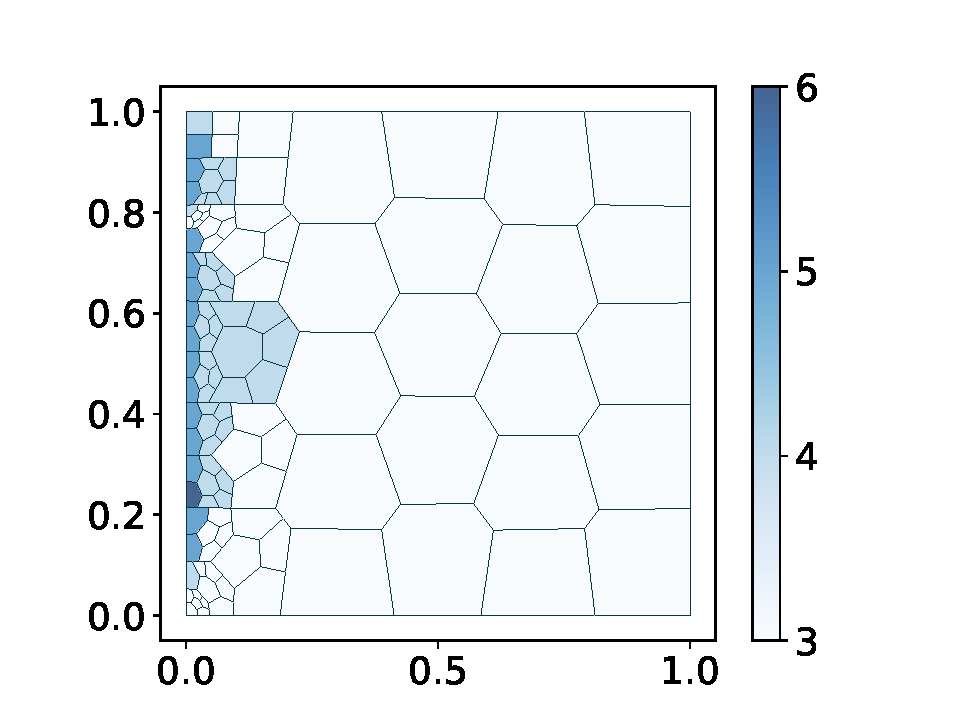
\includegraphics[width=5.5cm]{meshes/adaptive/square_hp_5.pdf}
	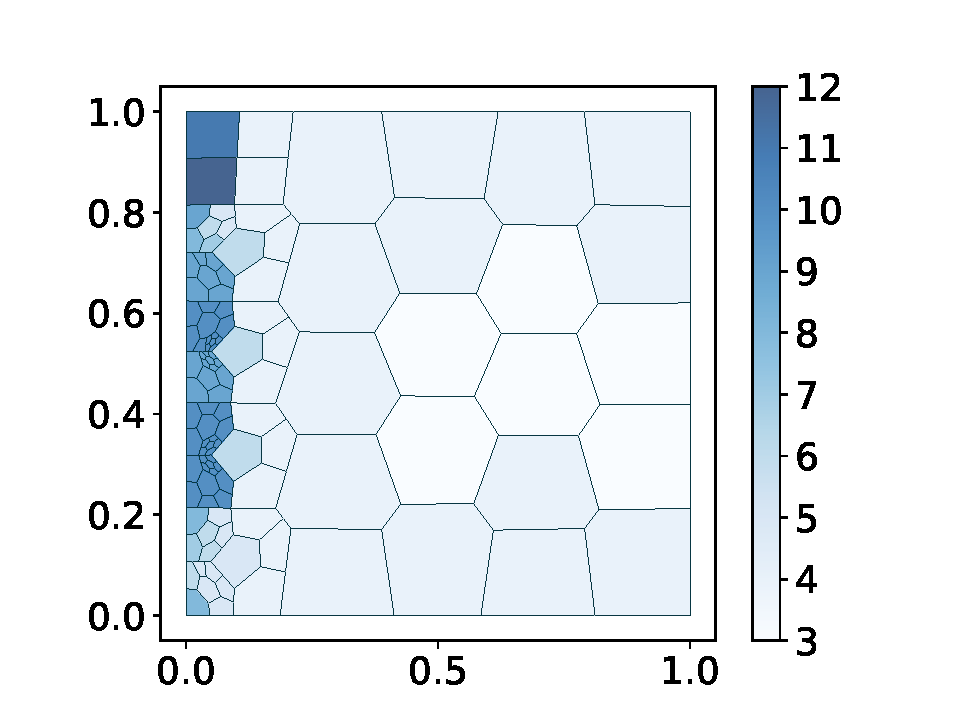
\includegraphics[width=5.5cm]{meshes/adaptive/square_hp_10.pdf}
    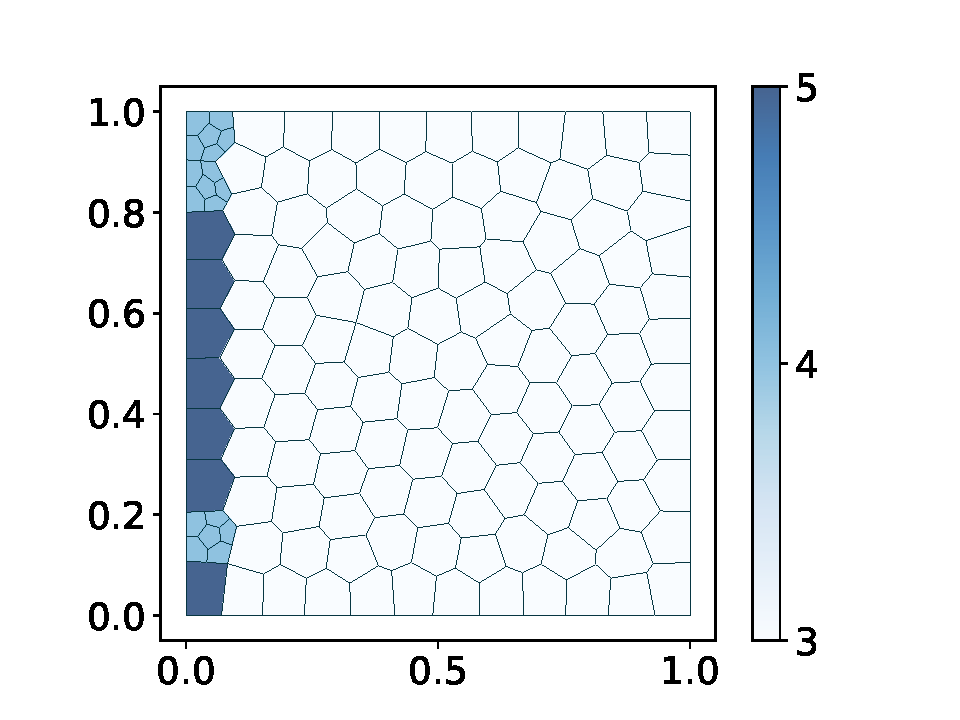
\includegraphics[width=5.5cm]{meshes/adaptive/square_hp_125_2.pdf}
	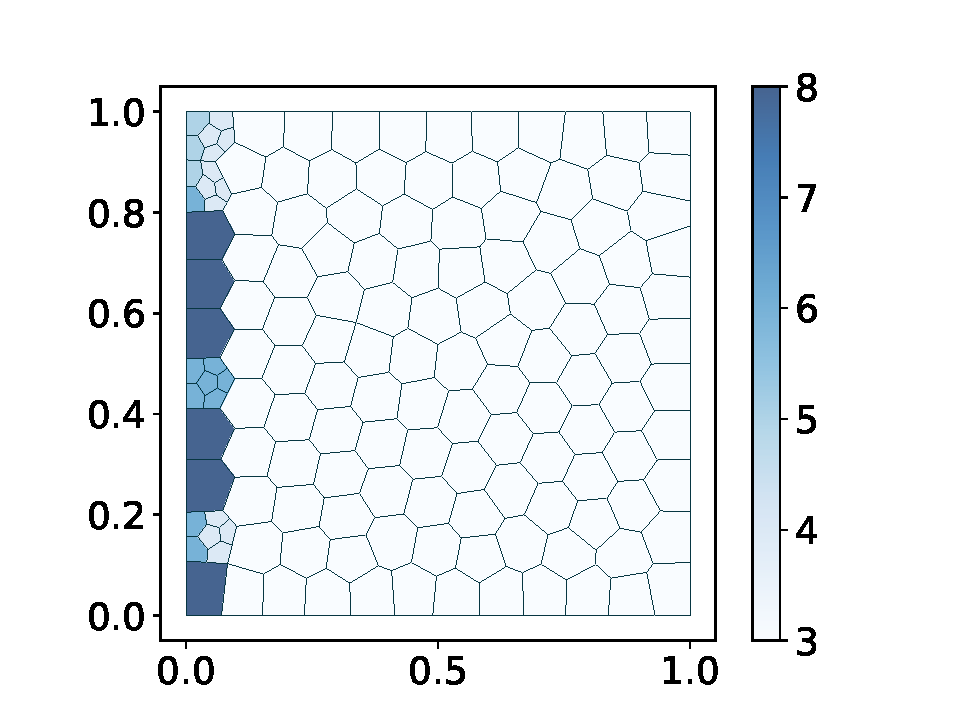
\includegraphics[width=5.5cm]{meshes/adaptive/square_hp_125_5.pdf}
	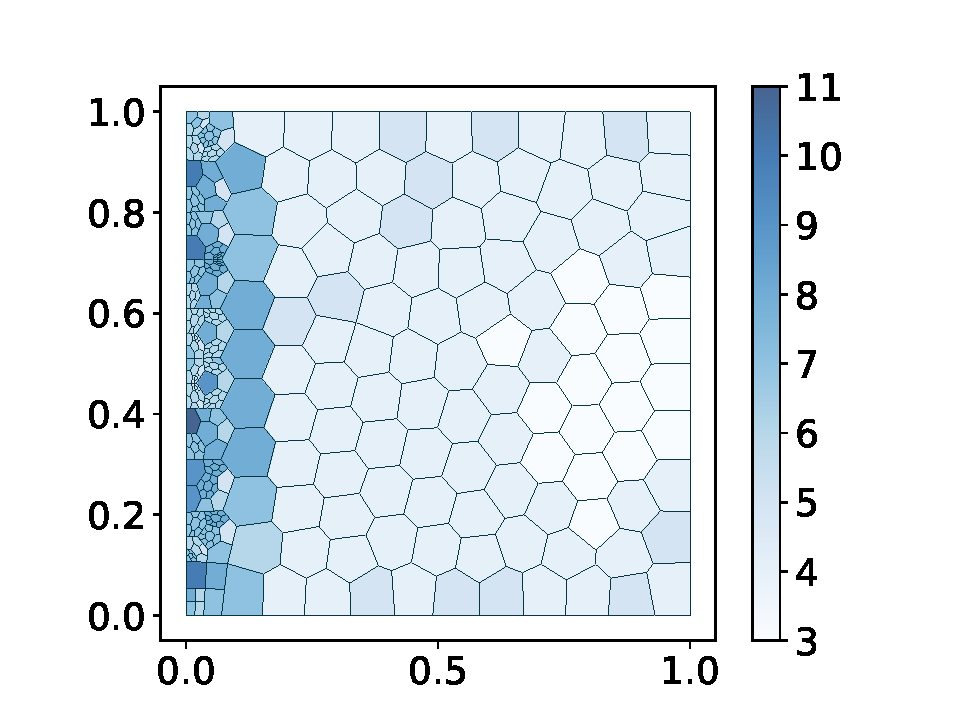
\includegraphics[width=5.5cm]{meshes/adaptive/square_hp_125_10.pdf}
	\caption{Square mesh after 2, 5, and 10 refinements. $k_0 = 3$, $N_0 = 25$ (top) and $N_0 = 125$ (bottom).}
\end{figure}

\begin{figure}[!ht]
	\centering
	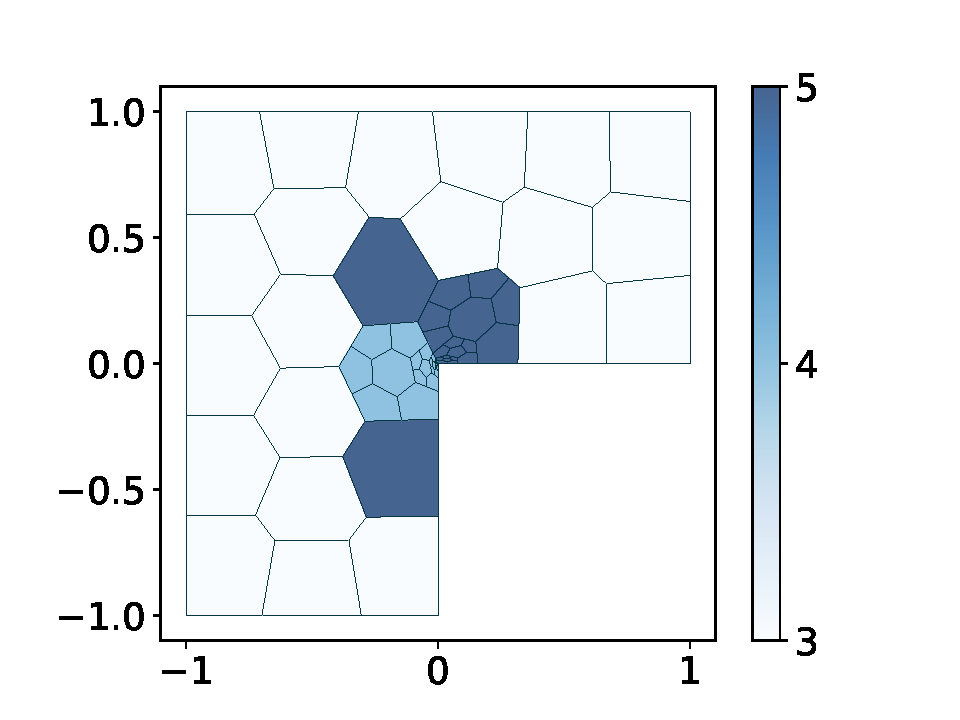
\includegraphics[width=5.5cm]{meshes/adaptive/lshape_hp_5.pdf}
	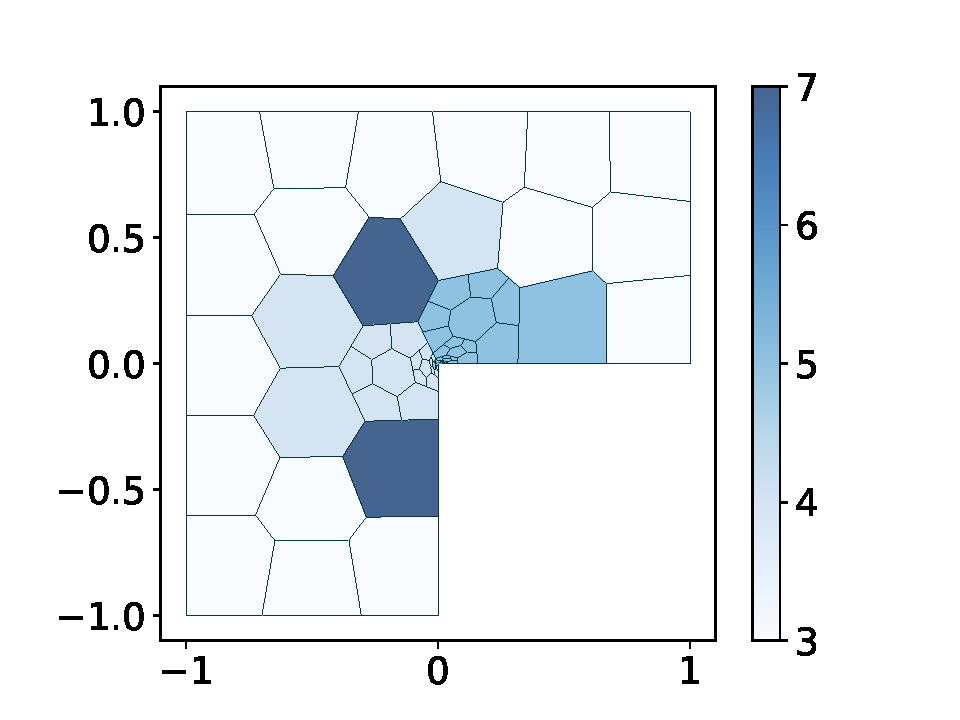
\includegraphics[width=5.5cm]{meshes/adaptive/lshape_hp_10.pdf}
	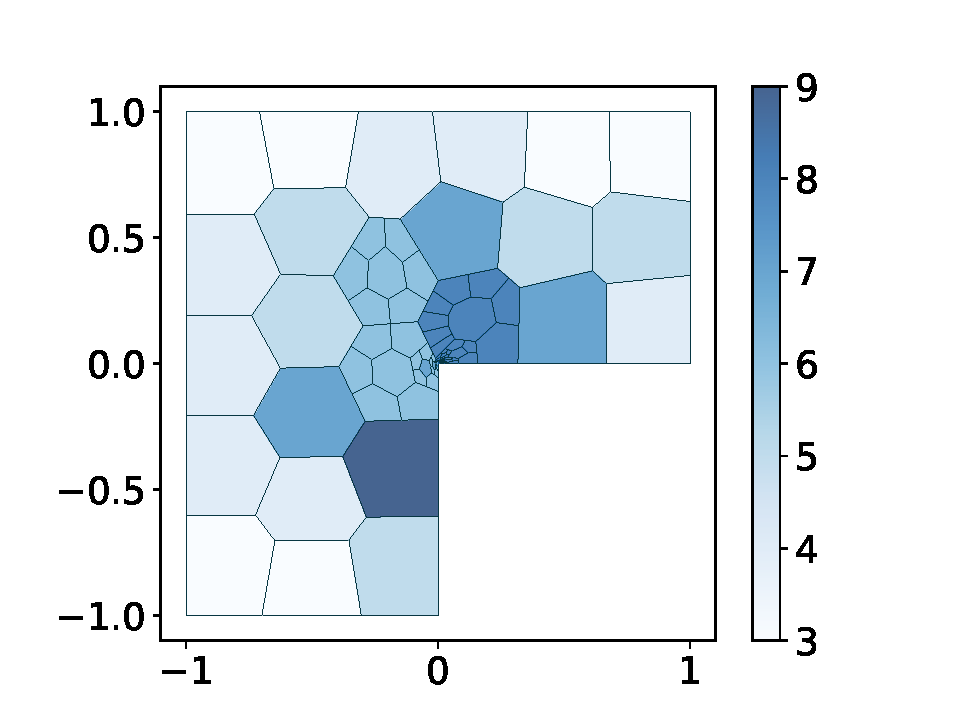
\includegraphics[width=5.5cm]{meshes/adaptive/lshape_hp_15.pdf}
    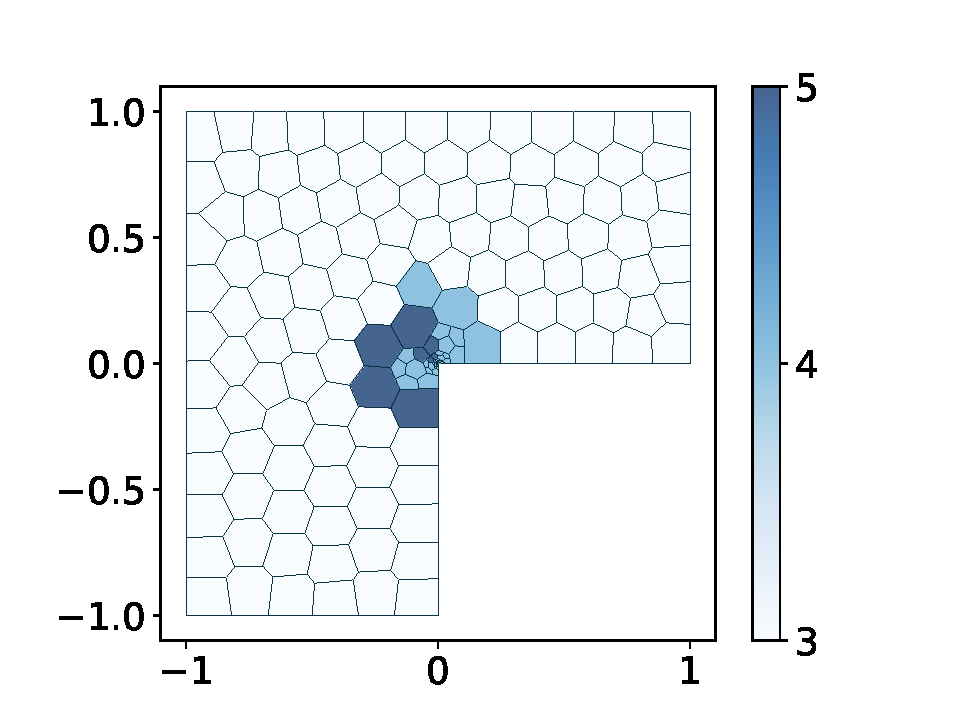
\includegraphics[width=5.5cm]{meshes/adaptive/lshape_hp_125_5.pdf}
	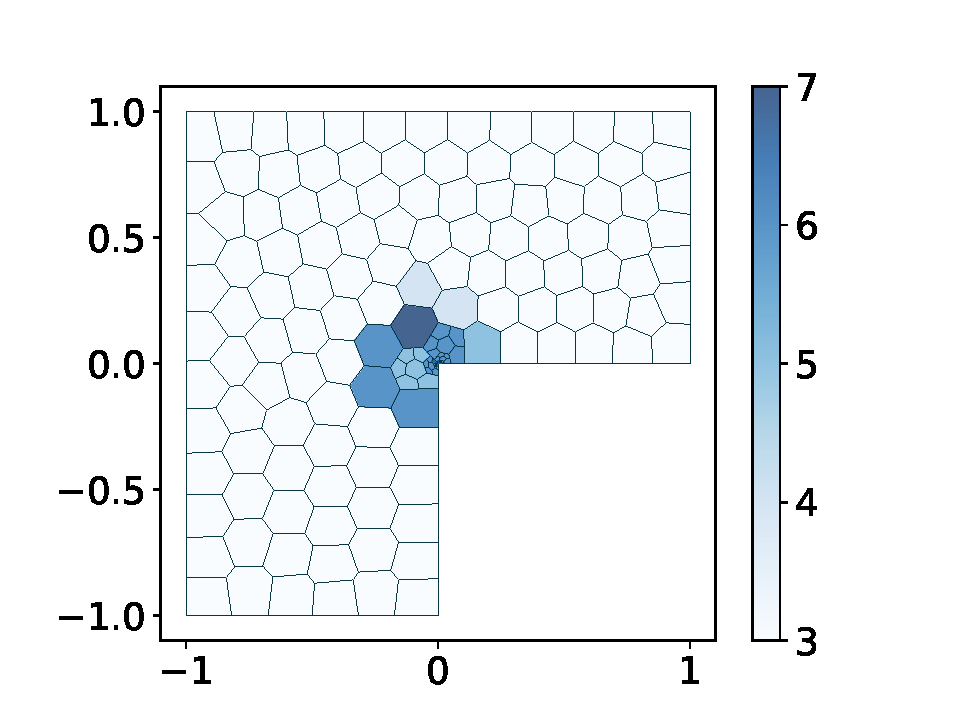
\includegraphics[width=5.5cm]{meshes/adaptive/lshape_hp_125_10.pdf}
	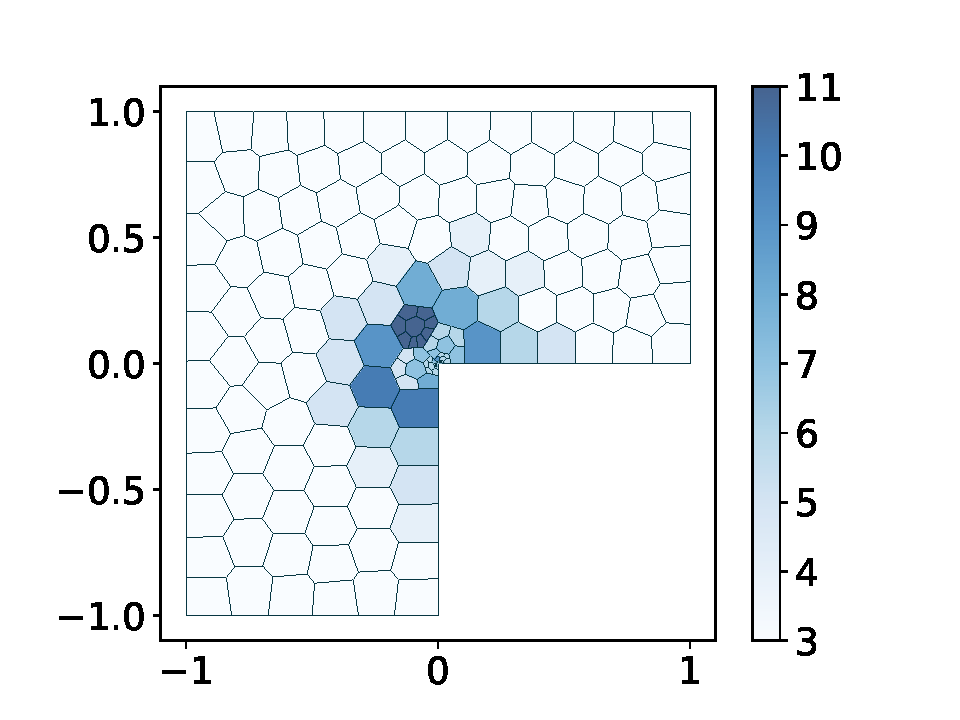
\includegraphics[width=5.5cm]{meshes/adaptive/lshape_hp_125_15.pdf}
	\caption{L-shaped mesh after 5, 10, and 15 refinements. $k_0 = 3$, $N_0 = 25$ (top) and $N_0 = 125$ (bottom).}
\end{figure}

\newpage
\subsection{\textit{h-refinement} versus \textit{hp-refinement}}

The final step in implementing \textit{hp-adaptivity} is to compare the results of \textit{h-refinement} and \textit{hp-refinement}. One approach is to choose a basic starting mesh, using a low polynomial degree and a small number of elements.

\begin{figure}[!ht]
    \begin{subfigure}[b]{0.45\textwidth}
		% HP v DOFs template for TikZ.

\begin{tikzpicture}
\begin{axis}[
    xlabel={$DOFs^{1/2}$}, % Edit if needed.
    legend pos=north east,
    ymode=log
]

\addplot[solarized-base02, mark=*] coordinates {(8.660254037844387,2.1812) (10.954451150103322,2.04967) (14.071247279470288,2.93871) (15.968719422671311,3.13011) (17.916472867168917,2.76594) (20.273134932713294,2.26584) (22.315913604421397,1.89116) (23.93741840717165,1.76002) (27.2213151776324,1.48665) (30.740852297878796,1.49861) (32.17141588429082,1.49545) (35.02855977627399,1.39444) (41.1703777004778,1.3207) (51.43928459844674,1.11561) (58.40376700179535,0.986776) (68.38859554048467,0.782051) (80.87026647662292,0.669326) (91.27431182978046,0.619557) (103.50362312499017,0.558376) (123.75378782081783,0.514557) (144.9137674618944,0.424657) (167.88388844674762,0.373345)};
\addlegendentry{\textit{h-refinement}}

\addplot[\accentcolor, mark=*] coordinates {(8.660254037844387,2.1812) (9.486832980505138,5.48286) (10.488088481701515,8.28706) (17.175564037317667,6.37634) (21.6794833886788,3.07509) (25.96150997149434,1.71936) (30.903074280724887,1.06513) (36.4828726939094,0.935197) (37.72267222772003,0.3543) (43.0,0.173769) (44.68780594300866,0.204124) (49.66890375275057,0.0514923) (54.76312628037227,0.0282501) (60.63827174318213,0.0146515) (64.77653896280658,0.0079507)};
\addlegendentry{\textit{hp-refinement}}

\end{axis}
\end{tikzpicture}
	\end{subfigure}
	\hfill
	\begin{subfigure}[b]{0.45\textwidth}
		% HP v DOFs template for TikZ.

\begin{tikzpicture}
\begin{axis}[
    xlabel={$DOFs^{1/3}$}, % Edit if needed.
    legend pos=north east,
    ymode=log
]

\addplot[solarized-base02, mark=*] coordinates {(4.217163326508746,0.191755) (4.805895533705332,0.173165) (5.484806552432618,0.17539) (6.162240147749038,0.164783) (7.054004063162272,0.138814) (7.989569740454012,0.127309) (9.39024187300355,0.103252) (10.297715269155368,0.0927241) (11.221408880627516,0.0789875) (12.21822948857921,0.073464) (14.067699311995325,0.0602545) (16.126599805218184,0.0536889) (17.386751706878687,0.0492177) (18.66925275961817,0.0425939) (20.31339680458661,0.0374376) (22.29090233304798,0.0313125) (23.651205489315725,0.028713) (23.918123773897065,0.0278557) (26.648390254618004,0.0253127) (27.653467034596552,0.0247917) (27.769363970258176,0.0242055) (30.87951848068366,0.0213387)};
\addlegendentry{\textit{h-refinement}}

\addplot[\accentcolor, mark=*] coordinates {(4.217163326508746,0.191755) (4.672328728355259,0.255398) (5.0132979349645845,0.248801) (5.383212612087283,0.291174) (5.708267473384861,0.328607) (6.832771452246442,0.404871) (9.878530490026034,0.485699) (12.69507321245234,0.659013) (14.55901434377428,0.230073) (15.921490395218942,0.122269) (16.623800957486996,0.098664) (17.340316055801914,0.0495985) (17.714635665253457,0.0495794) (18.10839938601742,0.0283923) (18.477938151928672,0.0126687) (19.10925056502305,0.00835058) (20.20211721754757,0.00451385) (20.823924640400417,0.00216312) (21.4106622851008,0.00136207) (22.436197851201577,0.00072339)};
\addlegendentry{\textit{hp-refinement}}

\end{axis}
\end{tikzpicture}
	\end{subfigure}
    \caption{$DG$ error versus $DOFs^{1/2}$ (left) and $DOFs^{1/3}$ (right) on sequences of \textit{h-adaptively} (black) and \textit{hp-adaptively} (blue) refined meshes over a square (left) and an L-shaped domain (right). $k_0 = 1$, $N_0 = 25$.}
\end{figure}

This comparison highlights the superiority of the \textit{hp-adaptive} method over the \textit{h-adaptive} approach, greatly reducing the error while utilizing significantly fewer $DOFs$.

\newpage
\subsection{A code snippet}

Here's a snippet to illustrate the \textit{hp-adaptive} mesh refinement from the user's perspective:

\lstinputlisting[style=cpp, firstline=11]{../snippets/hp_refine.cpp}